\documentclass{beamer}	% Compile at least twice!
%\setbeamertemplate{navigation symbols}{}
\usetheme{default}
\usecolortheme{whale}
%\useinnertheme{rectangles}
%\useoutertheme{infolines}
%\useoutertheme[title,section,subsection=true]{smoothbars}
 
% -------------------
% Packages
% -------------------
\usepackage{
	amsmath,			% Math Environments
	amssymb,			% Extended Symbols
	enumerate,		    % Enumerate Environments
	graphicx,			% Include Images
	lastpage,			% Reference Lastpage
	multicol,			% Use Multi-columns
	multirow,			% Use Multi-rows
	pifont,			    % For Checkmarks
	stmaryrd,			% For brackets
	threeparttable,		% For tables
	pgf-pie,			% PIE CHART
	caption
}
\usepackage[english]{babel}


% -------------------
% Colors
% -------------------
\definecolor{UniOrange}{RGB}{212,69,0}
\definecolor{UniGray}{RGB}{62,61,60}
%\definecolor{UniRed}{HTML}{B31B1B}
%\definecolor{UniGray}{HTML}{222222}
%\setbeamercolor{title}{fg=UniGray}
%\setbeamercolor{frametitle}{fg=UniOrange}
%\setbeamercolor{structure}{fg=UniOrange}
%\setbeamercolor{section in head/foot}{bg=UniGray}
%\setbeamercolor{author in head/foot}{bg=UniGray}
%\setbeamercolor{date in head/foot}{fg=UniGray}
%\setbeamercolor{structure}{fg=UniOrange}
%\setbeamercolor{local structure}{fg=black}
\beamersetuncovermixins{\opaqueness<1>{0}}{\opaqueness<2->{15}}

\setbeamertemplate{caption}[numbered]
% -------------------
% Fonts & Layout
% -------------------
\useinnertheme{default}
%\usefonttheme{serif}
\usepackage{palatino}
%\setbeamerfont{title like}{shape=\scshape}
%\setbeamerfont{frametitle}{shape=\scshape}
\setbeamertemplate{itemize items}[circle]
%\setbeamertemplate{enumerate items}[default]


% -------------------
% Commands
% -------------------

% Special Characters
\newcommand{\N}{\mathbb{N}}
\newcommand{\Z}{\mathbb{Z}}
\newcommand{\Q}{\mathbb{Q}}
\newcommand{\R}{\mathbb{R}}
%\newcommand{\C}{\mathbb{C}}

% Math Operators
\DeclareMathOperator{\im}{im}
\DeclareMathOperator{\Span}{span}

% Special Commands
\newcommand{\pf}{\noindent\emph{Proof. }}
\newcommand{\ds}{\displaystyle}
\newcommand{\defeq}{\stackrel{\text{def}}{=}}
\newcommand{\ov}[1]{\overline{#1}}
\newcommand{\ma}[1]{\stackrel{#1}{\longrightarrow}}
\newcommand{\twomatrix}[4]{\begin{pmatrix} #1 & #2 \\ #3 & #4 \end{pmatrix}}


% -------------------
% Tikz & PGF
% -------------------
\usepackage{tikz}
\usepackage{tikz-cd}
\usetikzlibrary{
	calc,
	decorations.pathmorphing,
	matrix,arrows,
	positioning,
	shapes.geometric
}
\usepackage{pgfplots}
\pgfplotsset{compat=newest}


% -------------------
% Theorem Environments
% -------------------
\theoremstyle{plain}
\newtheorem{thm}{Theorem}[section]
\newtheorem{prop}{Proposition}[section]
\newtheorem{lem}{Lemma}[section]
\newtheorem{cor}{Corollary}[section]
\theoremstyle{definition}
\newtheorem{ex}{Example}[section]
\newtheorem{nex}{Non-Example}[section]
\newtheorem{dfn}{Definition}[section]
\theoremstyle{remark}
\newtheorem{rem}{Remark}[section] 
\numberwithin{equation}{section}


% -------------------
% Fonts
% -------------------
\usepackage{ctex}
\usepackage{fontspec}

\setmainfont[Ligatures=TeX]{Times New Roman}
\setsansfont{Arial}
\setmonofont{Consolas}
 
\setCJKmainfont[BoldFont={等线},ItalicFont={宋体}]{宋体}
\setCJKsansfont{等线}
\setCJKmonofont{宋体}

%\setCJKfamilyfont{song}{宋体}
%\setCJKfamilyfont{pingfang}{微软雅黑}
%\setCJKfamilyfont{huasong}{宋体}
%\setCJKfamilyfont{dongqinghei}{黑体}
%\setCJKfamilyfont{hei}{等线}
%\setCJKfamilyfont{hwfangsong}{仿宋}
%\setCJKfamilyfont{huawenheiti}{等线}
%\setCJKfamilyfont{kaiti}{楷体}


%\newcommand*{\songti}{\CJKfamily{song}} % 宋体
%\newcommand*{\heiti}{\CJKfamily{hei}} % 黑体
%\newcommand*{\dqhei}{\CJKfamily{dongqinghei}} % 冬青黑体
%\newcommand*{\pfhei}{\CJKfamily{pingfang}} % 苹方黑体
%\newcommand*{\hwsong}{\CJKfamily{huasong}}    % 华文宋
%\newcommand*{\fangsong}{\CJKfamily{hwfangsong}}    % 华文仿宋
%\newcommand*{\hwhei}{\CJKfamily{huawenheiti}}    % 华文黑体
%\newcommand*{\kai}{\CJKfamily{kaiti}}    % 楷体




% -------------------
% Title Page
% -------------------
\title{\textcolor{white}{题目Impacts of Internet Access on Food and Nutrition Consumption}}
\subtitle{\textcolor{white}{Evidence from Rural China}}  
\author{\textbf{韩昕儒} and Xiudong Wang} 
\institute[IAED, CAAS]{Institute of Agricultural Economics and Development (IAED), \\ Chinese Academy of Agricultural Sciences (CAAS) }
\date{IAMO Forum 2020 \\ June 24, 2020} 


% -------------------
% Content
% -------------------
\begin{document}


% Title Page
\begin{frame}
\titlepage
\end{frame}



% Motivation
\section{Motivation}

\subsection {Backgrond}
\begin{frame}
	\linespread{1.2}
	\begin{block}{Internet in China}
		\textbf{Largest}: China already has the largest population of Internet user in the world.\\
		\vspace{.1cm}
		\textbf{225/855}: The number of Chinese Internet users have reached 855 million by the August, 2019, and 225 million of them are rural residents (CNNIC, 2019). 
	\end{block}
	\centering
	\begin{figure}
		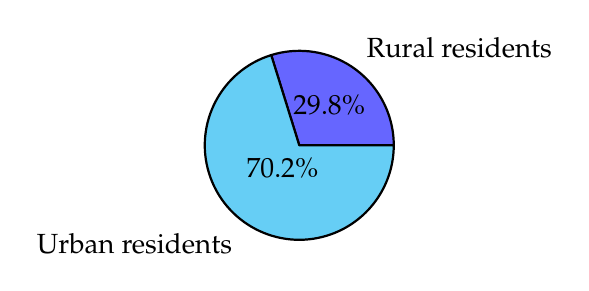
\begin{tikzpicture}[scale=0.4] % Tikz environment
			\pie
			 {29.8/Rural residents, 70.2/Urban residents} % it is essential to recheck that the sum of all the components mentioned should be 100%. Otherwise, Latex will leave the left percentage, blank.
		\end{tikzpicture}
		\caption{Composition of Chinese Internet Users}
	\end{figure}
\end{frame}

\subsection {Lit. Rev.}  
\begin{frame}
	\linespread{1.2}
	\begin{block}{Internet and Individual Behaviors}
		\textbf{I}. The Internet has been regarded as the most important channel of information acquisition (Riaz et al., 2018).\\
		\vspace{.1cm}
		\textbf{II}. The information on Internet may affect the individual behaviors: environment information (Zhang et al, 2020), health information (Chen et al., 2019; Estacio et al., 2019), agricultural information (Fan and Garcia, 2018; Deng et al., 2019), e‐commerce promotion (Ma et al., 2019). 
	\end{block}
\end{frame}

\subsection {Research Questions}   
\begin{frame}
	\linespread{1.2}
	\begin{block}{Research Questions}
		\textbf{I}. What is the difference of food/nutrition consumption between rural residents with/without Internet access? \\
		\vspace{.1cm}
		\textbf{II}. What is the potential channel that the Internet influences food/nutrition consumption? \\
	\end{block}
\end{frame}

\subsection {Countributions}    
\begin{frame}
	\linespread{1.2}
	\begin{block}{Contributions}
		\textbf{I}. Evaluating the impacts of Internet access on food/nutrition consumption. \\
		\vspace{.1cm}
		\textbf{II}. Provide policy implications that would be helpful for developing food security strategies in rural areas. 
	\end{block}
\end{frame}


% Framework
\section{Framework}

\subsection {Intro. PSM}
\begin{frame}
	\textbf{Methodology: Propensity Score Matching (PSM)} \\
	\begin{itemize}
		\item Counterfactual method (Pseudo-experiment)
		\item \textbf{Correct for selection bias}: residents with/without Internet access may have different characters, which might affect food/nutrition consumption
		\item Control for all major factors that may affect food/nutrition consumption
		\item Estimate the average treatment effect (ATT) by matching individuals from two groups with similar score
		\item \textbf{Treatment: Internet access}
	\end{itemize}
	\begin{block}{Two Groups}
		\textbf{Treatment Group}: IAs: rural residents with Internet access \\
		\textbf{Control Group}: Non-IAs: rural residents without Internet access
	\end{block}
\end{frame}

\subsection {PSM Steps}
\begin{frame}
	\textbf{Methodology: Propensity Score Matching (PSM)} \\
	\linespread{1.2}
	\begin{block}{Step I}
		Construct a Probit model to predict the probability of a rural resident to access the Internet
	\end{block}
		\[p(X_i)=prob(\Gamma_i=1|X_i)=\int_{-\infty}^{\beta^{'}X_i}\phi(z)dz=\phi(\beta^{'}X_i)\]
	\begin{itemize}
		\item \(\Gamma_i=1\):IAs\\
		\(\Gamma_i=0\): Non-IAs
		\item \(X_i\): a vector of relevant factors correlated with Internet access, including HH Sex, HH Age, HH Education, Income per capita, Children rate, Senior rate and Avg. food price.
		\item \(\beta\): parameters to be estimated
	\end{itemize}
\end{frame}

\begin{frame}
	\textbf{Methodology: Propensity Score Matching (PSM)} \\
	\linespread{1.2}
	\begin{block}{Step II}
		Match samples based on the propensity score
	\end{block}
		Apply different algorithms, including:\\
	\begin{itemize}
		\item Nearest-neighbor matching algorithm
		\item Kernel-matching algorithm
		\item Radius-matching algorithm
		\item \dots
	\end{itemize}
\end{frame}

\begin{frame}
	\textbf{Methodology: Propensity Score Matching (PSM)} \\
	\linespread{1.2}
	\begin{block}{Step III}
		Calculate ATT based on the matched samples: \\
		$ATT=E[y_i^T-y_i^C|\Gamma_{i}=1,p(X_i)]$
	\end{block}
	\begin{itemize}
		\item \(\Gamma_i=1\): IAs;
		\item \(T\): treatment group, \(C\): control group
	\end{itemize}
\end{frame}

\subsection {Two Conditions}
\begin{frame}
	\textbf{Methodology: Propensity Score Matching (PSM)} \\
	\underline{Two conditions} \\
	\begin{itemize}
		\item To ensure the matching estimators correctly identify the treatment effects (Rosenbaum and Rubin, 1983): 
		\item \textbf{Condition I}: \textbf{Matching balancing}: households with the same propensity score have similar or at least not so different characteristics. 
		\item \textbf{Condition II}: \textbf{Conditional independence}: the treatment assignment is independent of the potential outcomes after controlling for the observed covariates.
	\end{itemize}
\end{frame}

% Data
\section{Data}

\subsection {Data}
\begin{frame}
	\textbf{Data source} \\
	\underline{China Rural Micro-Econ. Data of IAED, CAAS}
	\begin{itemize}
		\item 48,058 rural households in Hebei, Jilin, Fujian, Shandong Henan, Yunnan, Shaanxi and Xinjiang provinces.
		\item 2012-2018 unbalanced panel data.
		\item Food consumption of grain, livestock products (-red meats, poultry, egg and milk), edible oil, vegetable and fruit.
		\item From food consumption to nutrition consumption: based on \emph{China Food Composition}.
		\item Nutrition per capita: Energy intake (EI, kcal/day), Carbohydrate (g/day), Fat (g/day) and Protein (g/day).
\end{itemize}
\end{frame}

\subsection {Identification}
\begin{frame}
	\begin{block}{How to identify treatment/control groups?}
		\linespread{1.2}
		\textbf{Internet access}: Own \(\geq1\) computer(s).\\
		\vspace{.1cm}
		\textbf{computer or mobile phone?}: Since there are lots of 2G mobile phones in rural China, computer is a better proxy variable of Internet access. 
	\end{block}
\end{frame}

\subsection {Statistic Description}
\begin{frame}
	\textbf{Statistic Description}: Nutrition Consumption \\
	\underline{Rural residents with Internet access have more energy intake.} \\
	\centering
	\begin{table}[]
		\caption{Summary Statistics of Nutrition Consumption}
		\resizebox{\textwidth}{!}{%
		\begin{tabular}{lrrrr}
		\hline
		\multicolumn{1}{c}{Variables} & \multicolumn{1}{c}{Full sample} & \multicolumn{1}{c}{(1) IAs} & \multicolumn{1}{c}{(2) Non-IAs} & \multicolumn{1}{c}{\textcolor{red}{(1)-(2) Diff.}}   \\
		\hline
		EI (kcal/day)            & 1478.62(975.68)                 & 1522.50(1014.06)            & 1421.66(920.48)                 & \textcolor{red}{100.80*(19.49) }                 \\
		Carbohydrate (g/day)          & 198.75(154.41)                  & 196.14(153.02)              & 202.13(156.14)                  & -5.99(3.089)     					                \\
		Fat (g/day)                   & 60.89(47.33)                    & 66.05(51.15)                & 54.18(40.89)                    & \textcolor{red}{11.86*(0.940)  }                 \\
		Protein (g/day)               & 37.55(25.91)                    & 39.31(27.35)                & 35.27(23.71)                    & \textcolor{red}{4.04*(0.517)   }                \\
		\hline
		Sample size          & 10166           & 5743             & 4423            &                 \\
		\hline
		\end{tabular}
		}
		\begin{tablenotes}
			\item \tiny{Standard deviations/errors in parentheses.}
			\item \tiny{* indicates the significance level at 5\%.}
		\end{tablenotes}		
	\end{table}
\end{frame}

% Results
\section{Results}
\subsection {Matching Quality}
\begin{frame}
	\textbf{Distributions of Propensity Score/Matching Balancing}: High Matching Quality \\
	\begin{columns}
	\begin{column}{0.5\textwidth}
	\begin{figure}
	\includegraphics[scale=0.225]{fa.png}
	\caption{Before NN(5) matching}
	\end{figure}
	\end{column}
	\begin{column}{0.5\textwidth}
	\begin{figure}
	\includegraphics[scale=0.225]{fb.png}
	\begin{footnotesize}
	\caption{After NN(5) matching}
	\end{footnotesize}
	\end{figure}
	\end{column}
	\end{columns}
\end{frame}

\subsection {Matching Results}
\begin{frame}
	\textbf{Full Sample}: Positive Nutrition Impacts \\
	\underline{Energy intake of IAs is \textcolor{red}{4.75\%} more than that of the Non-IAs.} \\
	\centering
	\begin{table}[]
		\caption{Effects of Internet Access on Nutrition Consumption: Full Sample}
		\resizebox{\textwidth}{!}} \\
			\hline
			EI             & 1656.34                     & 1581.30                         & 75.04*                          & \textcolor{red}{4.75*}                         \\
			Carbohydrate         & 213.64                      & 217.16                          & -3.52                           & -1.62                        \\
			Fat                  & 71.73                       & 63.80                           & 7.94*                           & \textcolor{red}{12.45*}                        \\
			Protein              & 42.77                       & 38.85                           & 3.92*                           & \textcolor{red}{10.08*}                        \\
			\hline
		\end{tabular}%
		}
		\begin{tablenotes}
			\item \tiny{units of EI=kcal/day; units of other variables=g/day}
			\item \tiny{ATT is calculated based on 5 nearest-neighbor matching algorithm.}
			\item \tiny{* indicates the significance level at 5\%.}
		\end{tablenotes}		
	\end{table}
\end{frame}


\subsection {Heterogeneity}
\begin{frame}
	\textbf{Heterogeneity Check}: Income levels \\
	\underline{Energy intake impacts show an \textcolor{red}{U-shape} curve among different} \\ \underline{income levels.} \\
	\centering
	\begin{table}[]
		\caption{Effects of Internet Access on Nutrition Consumption: Income Levels (Change\%)}
		\resizebox{\textwidth}{!}{%
		\begin{tabular}{lrrrrr}
			\hline
			\multicolumn{1}{c}{Nutrition} & \multicolumn{1}{c}{Lowest Inc. Lev.} & \multicolumn{1}{c}{Lower Inc. Lev.} & \multicolumn{1}{c}{Medium Inc. Lev.} & \multicolumn{1}{c}{Higher Inc. Lev.} & \multicolumn{1}{c}{Highest Inc. Lev.} \\
			\hline
			EI              & \textcolor{red}{13.08*}                               & \textcolor{red}{4.46*}                               & \textcolor{red}{-4.99*}                               & \textcolor{red}{-0.37}                                & \textcolor{red}{12.09*}                                \\
			Carbohydrate         & 0.96                                 & -3.04                               & -12.33*                              & -7.50*                               & 10.26*                                \\
			Fat                  & 34.08*                               & 15.32*                              & 4.74*                                & 8.86*                                & 12.39*                                \\
			Protein              & 14.75*                               & 9.41*                               & 1.02                                 & 4.92*                                & 17.93*                                \\
			\hline
		\end{tabular}%
		}
		\begin{tablenotes}
			\item \tiny{ATT is calculated based on 5 nearest-neighbor matching algorithm.}
			\item \tiny{* indicates the significance level at 5\%.}
		\end{tablenotes}		
	\end{table}
\end{frame}

\subsection {Robustness Check}
\begin{frame}
	\textbf{Robustness Check/Conditional Independence} \\
	\underline{Estimated impacts are robust to alternative matching algorithms.} \\
	\centering
	\begin{table}[]
		\caption{Effects of Internet Access on Nutrition Consumption: Different Matching Algorithms (Change\%)}
		%\resizebox{\textwidth}{!}{%
		\begin{tabular}{lrrrr}
			\hline
			\multicolumn{1}{c}{Nutrition} & \multicolumn{1}{c}{\textcolor{red}{NN(5)}} & \multicolumn{1}{c}{NN(1)} & \multicolumn{1}{c}{Kernel} & \multicolumn{1}{c}{LLR} \\
			\hline
			EI              & \textcolor{red}{4.75*}                               & 5.51*                               & 4.68*                                                              & 3.83*                                \\
			Carbohydrate         & \textcolor{red}{-1.62}                                 & -0.80                               & -1.70                                                            & -2.03                                \\
			Fat                  & \textcolor{red}{12.45*}                               & 12.82*                              & 12.31*                                                            & 10.53*                                \\
			Protein              & \textcolor{red}{10.08}                                & 11.73*                               & 10.36*                                                           & 9.81*                                \\
			\hline
		\end{tabular}%
		%}
		\begin{tablenotes}
			\item \tiny{NN(5)=5 nearest-neighbor; NN(1)=1 nearest-neighbor; LLR=local linear regression.}
			\item \tiny{* indicates the significance level at 5\%.}
		\end{tablenotes}		
	\end{table}
\end{frame}


% Discussion
\section{Discussion}
\subsection {Potential Channels}
\begin{frame}
	\linespread{1.2}
	\begin{block}{Potential Channels}
		\textbf{Channel I-Non-staple food consumption}: Internet may only affect non-staple food consumption. \\
		\vspace{.1cm}
		\textbf{Channel II-Lower prices}: One of the biggest advantage of online shopping is the low prices. \\
		\vspace{.1cm}
		\textbf{Channel III-Expenditure preference}: residents with Internet access may have have stronger willingness to consume. \\
	\end{block}
\end{frame}


\begin{frame}
	\textbf{Channel I-Non-staple food consumption}: Proved \\
	\underline{Internet only affects the non-staple food consumption.} \\
	\centering
	\begin{table}[]
		\caption{Effects of Internet Access on Food Consumption}
		%\resizebox{\textwidth}{!} & \multicolumn{1}{c}{Food} & \multicolumn{1}{c}{ATT Change\%}  \\
			\hline
			\textcolor{red}{Staple food} & \textcolor{red}{0.21}   & Poultry   & 12.86* \\
			Edible oil  & 8.93*  & Fish      & 50.74* \\
			Meat        & 31.55* & Vegetable & 11.57* \\
			Egg         & 14.98* & Fruit     & 27.99* \\
			Milk        & 36.41* &           &        \\
			\hline
		\end{tabular}%
		%}
		\begin{tablenotes}
			\item \tiny{ATT is calculated based on 5 nearest-neighbor matching algorithm.}
			\item \tiny{* indicates the significance level at 5\%.}
		\end{tablenotes}		
	\end{table}
\end{frame}


\begin{frame}
	\textbf{Channel II-Lower prices}: Partly Proved \\
	\underline{Lower prices of edible oil, meat, egg and milk.} \\
	\centering
	\begin{table}[]
		\caption{Effects of Internet Access on Food Prices}
		%\resizebox{\textwidth}{!} & \multicolumn{1}{c}{Food} & \multicolumn{1}{c}{ATT Change\%}  \\
			\hline
			\textcolor{blue}{Staple food} & \textcolor{blue}{1.37}    & \textcolor{red}{Poultry}   & \textcolor{red}{9.16*}  \\
			Edible oil  & -5.90*  & \textcolor{blue}{Fish}      & \textcolor{blue}{-1.11}  \\
			Meat        & -3.41*  & \textcolor{red}{Vegetable} & \textcolor{red}{4.53*}  \\
			Egg         & -6.58*  & \textcolor{red}{Fruit}     & \textcolor{red}{10.15*} \\
			Milk        & -13.44* &           &        \\
			\hline
		\end{tabular}%
		%}
		\begin{tablenotes}
			\item \tiny{ATT is calculated based on 5 nearest-neighbor matching algorithm.}
			\item \tiny{* indicates the significance level at 5\%.}
		\end{tablenotes}		
	\end{table}
\end{frame}

\begin{frame}
	\textbf{Channel III-Expenditure preference}: Proved \\
	\underline{The total expenditure of the IAs is \textcolor{red}{34.64\%} higher.} \\
	\small{Since the income has been controled, there is no difference in income between the two groups after matching.} \\
	\centering
	\begin{table}[]
		\caption{Effects of Internet Access on Expenditures}
		\resizebox{\textwidth}{!} & \multicolumn{1}{c}{Food} & \multicolumn{1}{c}{ATT Change\%}  \\
			\hline
			Total expenditure     & 34.64*  & Trans. and comm. expenduture & 66.02* \\
			Food expenditure      & 31.92*  & \textcolor{red}{ECR expenditure}                 & \textcolor{red}{49.61}  \\
			Clothing expenditure  & 43.39*  & \textcolor{red}{HCMS expenditure}                & \textcolor{red}{5.96}   \\
			Residence expenditure & -10.98* & MGS expenditure                 & 62.22* \\
			\textcolor{red}{HFAS expenditure}      & \textcolor{red}{3.49}    &                                 &       \\
			\hline
		\end{tabular}%
		}
		\begin{tablenotes}
			\item \tiny{HFAS=household facilities, articles and services; ECR=education, caltural and recreation; HCMS=health care and medical services; MGS=miscellaneous goods and services.}
			\item \tiny{ATT is calculated based on 5 nearest-neighbor matching algorithm.}
			\item \tiny{* indicates the significance level at 5\%.}
		\end{tablenotes}		
	\end{table}
\end{frame}

\subsection {Conclusions and Policy Implications}
\begin{frame}
	\textbf{Conclusions} \\
	\begin{itemize}
		\item Internet access can increase nutrition consumption in addition to carbohydrates
		\item The impacts of Internet access on nutrition consumption have heterogeneity 
		\item Non-staple food consumption, lower prices and expenditure preference are the channels through which IA may affect nutrition consumption
	\end{itemize}
\end{frame}

\begin{frame}
	\textbf{Policy Implications} \\
	\begin{itemize}
	\item Though lack of health data, it's important for policy makes to increase the Internet access rate in rural areas and improve the nutritional level of rural residents
	\end{itemize}
\end{frame}

% Questions
\subsection {}
\begin{frame}
	\begin{block}{THANKS FOR YOUR ATTENTION!}
	Q\&A
	\end{block}
	\textbf{Xinru Han} \\
	Institute of Agricultural Economics and Development, CAAS \\
	Add.: 12 Zhongguancun S. St., Beijing 100081, China P.R. \\
	E-mail: hanxinru@caas.cn \\
\end{frame}


\end{document}